\chapter{Technische Umsetzung}
\label{chap:technUmsetzung}

	\section{Speicherung der Profildaten}
	\label{sec:speicherungProfildaten}
	
	Profildaten, die der Nutzer in der App eingibt, werden persistent gespeichert. Die Daten werden mit dem Flutter Plugin SQLFlite (\url{https://pub.dev/packages/sqflite}) gespeichert. Das Plugin speichert Daten in einer SQLite Datenbank.
	\\
	Profildaten werden bei jeder Änderung automatisch gespeichert. Hierzu gehört nicht nur das Laden neuer Daten, sondern auch das Verändern von Eingabevariablen und dem Kommentarfeld.
	\\
	Die Datenverwaltung basiert im wesentlichen auf zwei Komponenten:
	
	\begin{itemize}
		\item \textbf{Profilklasse (\textit{profile.dart}):} Die Profilklasse repräsentiert Profile, die in der App gespeichert werden können. Jedes Profil besteht dabei aus einer ID, einem Namen, dem letzten Änderungsdatum, der ID, mit der die Messung vom Server geladen wurde (falls die Messung nicht per QR-Code gescannt wurde), einem Satz von Messwerten, einem Satz von Simulationswerten und dem optionalen Kommentar.
		
		Die Klasse verfügt außerdem über die Methode \textit{toMap()}, die ein Profil in eine Map konvertiert, die dann in der Datenbank gespeichert werden kann.				

		\item \textbf{Datenbank-Hilfsklasse (\textit{database\_helpers.dart}):} Die Hilfsklasse stellt sämtliche Funktionalitäten zur Verfügung, die genutzt werden, um mit der SQLite Datenbank zu interagieren. Die Klasse verwaltet die Erstellung der Datenbank-Tabelle und kann Daten zur Datenbank hinzufügen, löschen und bestehende Daten aktualisieren.
		
	\end{itemize}

	\begin{figure}[H]
		\centering
		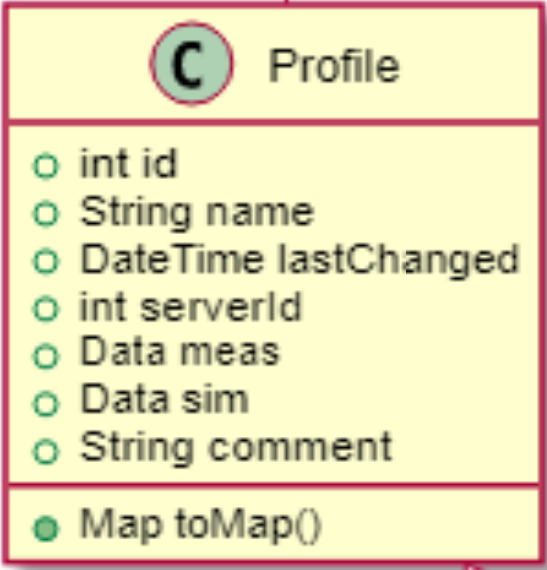
\includegraphics[width=0.5\textwidth]{../include/images/techdoc/profileClass}
		\label{img:commentTextfield}
		\caption{Aufbau der Profilklasse (\textit{profile.dart})}
	\end{figure}

	\begin{figure}[H]
		\centering
		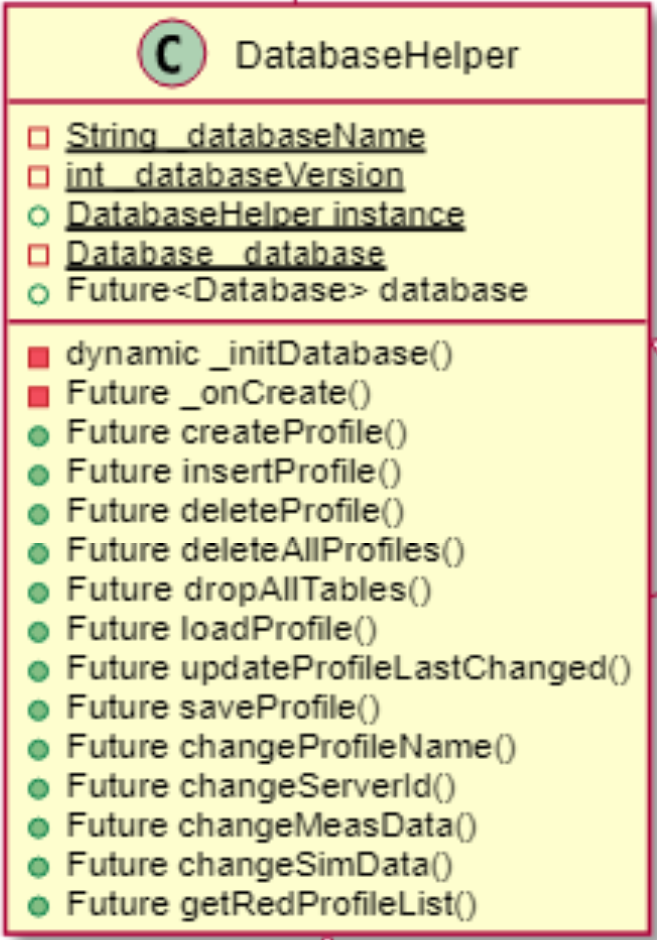
\includegraphics[width=0.5\textwidth]{../include/images/techdoc/dbHelperClass}
		\label{img:commentTextfield}
		\caption{Aufbau der Hilfsklasse (\textit{database\_helpers.dart})}
	\end{figure}

	
	\section{Speicherung der Einstellungen}
	\label{sec:speicherungEinstellungen}
	
	Die Daten zur Einstellung der App bestehen aus Präferenzen zur Sprache und zur Eingabemethode. Diese werden mithilfe des \textit{Shared preferences} Plugins (\url{https://flutter.dev/docs/cookbook/persistence/key-value}) persistent gespeichert. Da diese Daten nur sehr wenig Speicherplatz benötigen und eine Speicherung mithilfe von Shared preferences sehr einfach ist, wurde hierfür diese Technik gewählt.
	
	\section{Verwaltung des App-States}
	\label{sec:verwaltungAppState}
	
	Um den aktuellen Zustand der App über mehrere Ansichten verteilt nutzen zu können, wurde das \textit{scoped\_model} (\url{https://github.com/brianegan/scoped_model}) genutzt. Dieses ermöglicht es, ein aktuelles Modell des Zustandes an seine Kinderelemente weiterzugeben. Außerdem kann mit der statischen Methode \textbf{ScopedModel.of} das aktuelle Modell gefunden werden.
	\\
	Der Zustand, der in der App verwaltet werden muss, ist das aktuell ausgewählte Profil. In der Profilverwaltung werden lediglich Daten in der SQLite Datenbank verändert, dies verändert also noch nicht den Zustand der App. Sobald ein Nutzer ein Profil als aktuelles Profil auswählt, werden die Daten des entsprechenden Profils aus der Datenbank geholt und in den App-State geladen. Dadurch ist dann das aktuelle Profil auf jeder weiteren Ansicht verfügbar und kann genutzt werden. Weitere Daten sind für den Zustand der App im App-State nicht nötig.
	
	\section{Daten hinzufügen}
	\label{sec:addData}
	
	Um einem Profil neue Messdaten hinzuzufügen, können zwei Methoden genutzt werden:
	
	\begin{enumerate}
		\item \textbf{Scannen eines QR-Codes:} Der Nutzer scannt einen QR-Code ein, in dem jegliche Messdaten in Form eines JSON-Objektes encodiert sind. Zum Scannen und verarbeiten des QR-Codes wurde die Bibliothek \textit{barcode\_scan} (\url{https://pub.dev/packages/barcode_scan}) verwendet.
		\item \textbf{Laden der Daten vom Server:} Die Daten der Messung können des weiteren von einem Server geladen werden. Hierzu wird ein HTTP-Get-Request an den entsprechenden Server geschickt, der ebenfalls ein JSON-Objekt mit den Messdaten zurückgibt.
	\end{enumerate}	
	
	\section{Diagramme}
	\label{sec:charts}
	Um die Diagramme in der App anzeigen zu können wurde die Bibliothek \textit{charts\_flutter} (\url{https://github.com/google/charts/tree/master/charts_flutter}) benutzt. Diese ermöglicht es Diagramme darzustellen. Bei der Umsetzung der App wurden einige dieser Diagramme ausgewählt und in den einzelnen Diagrammdarstellung genutzt. Dabei wurden Achsen und Beschriftungen, wie in der Bibliothek beschrieben, individualisiert. Diese Diagrammdarstellungen können als Bausteine für die Diagrammseite gesehen werden, da jede Darstellung über eine Methode eine \textit{Row} zugibt, die den jeweiligen Baustein für die Diagrammseite darstellt. Dabei erben alle diese Diagrammdarstellungen von der Klasse \textit{ChartFactory}. Die \textit{ChartFactory} stellt Methoden bereit, um einheitliche Abstände und Überschriften zu gewährleisten.
	
	Es wurden zwei Diagrammdarstellungen programmiert. Das \textit{simOverviewChart} und das \textit{singleMeasChangeChart}. Das \textit{simOverviewChart} gibt eine Übersicht über die prozentuellen Veränderungen der Kennzahlen an. Dabei werden die Kennzahlen mit der betragsmäßig größten prozentuellen Veränderung genommen und angezeigt.
	Das \textit{singleMeasChangeChart} hingegen zeigt nur die Veränderung einer Kennzahl an. Dabei werden die absoluten Werte vor und nach der Simulation, sowohl als Zahl als auch als Säulendiagramm dargestellt.
	
	Um alle Diagrammdarstellungen zu ordnen, existiert die Klasse \textit{ChartInitializer}. Diese nutzt die einzelnen Diagrammdarstellungen, um daraus die Diagrammseite bauen zu können. Damit alle Diagramme auch auf Smartphones verschiedener Displaygrößen laufen kann, wird ein \textit{LayoutBuilder} verwendet. 